\begin{frame}[allowframebreaks, allowdisplaybreaks]
    \frametitle{B-Tree Operations---Insert (Example)}
    \newcounter{insert-example}
    \newcounter{insert-img-example}
    \newcounter{insert-step-example}[insert-example]
    \setcounter{insert-example}{0}
    \setcounter{insert-img-example}{0}
    \setcounter{insert-step-example}{0}
    % insert 1
    \stepcounter{insert-example}
    \stepcounter{insert-img-example}
	\stepcounter{insert-step-example}
    \begin{columns}
        \begin{column}{.47\textwidth}
            \inputminted[%
                highlightlines={1,2,3,4,5},%
                firstline=1,%
                lastline=11,%
                tabsize=1,%
                fontsize=\examplefnt,%
            ]{c}{resources/code/b_tree_insert.c}
        \end{column}
        \begin{column}{.5\textwidth}
            \examplefnt{%
                \begin{itemize}
                    \item Insert \arabic{insert-example}; Step \arabic{insert-step-example};
                    \item \hlght{tree=(*pag 0); new\_key=50; new\_object=(*50);}
                    \item finished; insert\_key;
                    \item \hlght{current\_node=(*pag 0);}
                \end{itemize}
            }
        \end{column}
    \end{columns}
    \begin{figure}[h!]
        \includegraphics[%
            width=0.45\linewidth,%
            page=\value{insert-img-example}%
        ]{resources/made/B-Trees_insert_example.pdf}
    \end{figure}
    \framebreak{}
    \stepcounter{insert-img-example}
	\stepcounter{insert-step-example}
    \stepcounter{insert-img-example}
    \begin{columns}
        \begin{column}{.47\textwidth}
            \inputminted[%
                highlightlines={6,7,8,9,10},%
                firstline=1,%
                lastline=11,%
                tabsize=1,%
                fontsize=\examplefnt,%
            ]{c}{resources/code/b_tree_insert.c}
        \end{column}
        \begin{column}{.5\textwidth}
            \examplefnt{%
                \begin{itemize}
                    \item Insert \arabic{insert-example}; Step \arabic{insert-step-example};
                    \item tree=(*pag 0); 
                        new\_key=50; 
                        new\_object=(*50);
                    \item finished; insert\_key;
                    \item current\_node=(*pag 0);
                \end{itemize}
            }
        \end{column}
    \end{columns}
    \begin{figure}[h!]
        \includegraphics[%
            width=0.45\linewidth,%
            page=\value{insert-img-example}%
        ]{resources/made/B-Trees_insert_example.pdf}
    \end{figure}
    \framebreak{}
    % Insert 2
    \stepcounter{insert-example}
    \stepcounter{insert-img-example}
	\stepcounter{insert-step-example}
    \begin{columns}
        \begin{column}{.47\textwidth}
            \inputminted[%
                highlightlines={6},%
                firstline=6,%
                lastline=6,%
                tabsize=1,%
                fontsize=\examplefnt,%
            ]{c}{resources/code/b_tree_insert.c}
            \inputminted[%
                highlightlines={13, 14},%
                firstline=13,%
                lastline=27,%
                tabsize=1,%
                fontsize=\examplefnt,%
            ]{c}{resources/code/b_tree_insert.c}
        \end{column}
        \begin{column}{.5\textwidth}
            \examplefnt{%
                \begin{itemize}
                    \item Insert \arabic{insert-example}; Step \arabic{insert-step-example};
                    \item \hlght{tree=(*pag 0); new\_key=20; new\_object=(*20);}
                    \item finished; insert\_key;
                    \item \hlght{current\_node=(*pag 0);}
                \end{itemize}
            }
        \end{column}
    \end{columns}
    \begin{figure}[h!]
        \includegraphics[%
            width=0.45\linewidth,%
            page=\value{insert-img-example}%
        ]{resources/made/B-Trees_insert_example.pdf}
    \end{figure}
    \framebreak{}
    \stepcounter{insert-img-example}
	\stepcounter{insert-step-example}
    \begin{columns}
        \begin{column}{.47\textwidth}
            \inputminted[%
                highlightlines={32,33,34,35,38,39},%
                firstline=30,%
                lastline=40,%
                tabsize=1,%
                fontsize=\examplefnt,%
            ]{c}{resources/code/b_tree_insert.c}
        \end{column}
        \begin{column}{.5\textwidth}
            \examplefnt{%
                \begin{itemize}
                    \item Insert \arabic{insert-example}; Step \arabic{insert-step-example};
                    \item tree=(*pag 0); new\_key=20; new\_object=(*20);
                    \item \hlght{finished=0; insert\_key=20; insert\_pt=(*20);}
                    \item current\_node=(*pag 0);
                    \item \hlght{i; start=0;}
                \end{itemize}
            }
        \end{column}
    \end{columns}
    \begin{figure}[h!]
        \includegraphics[%
            width=0.45\linewidth,%
            page=\value{insert-img-example},%
        ]{resources/made/B-Trees_insert_example.pdf}
    \end{figure}
    \framebreak{}
    \stepcounter{insert-img-example}
	\stepcounter{insert-step-example}
    \begin{columns}
        \begin{column}{.47\textwidth}
            \inputminted[%
                highlightlines={42,44,45,46,47},%
                firstline=41,%
                lastline=49,%
                tabsize=1,%
                fontsize=\examplefnt,%
            ]{c}{resources/code/b_tree_insert.c}
        \end{column}
        \begin{column}{.5\textwidth}
            \examplefnt{%
                \begin{itemize}
                    \item Insert \arabic{insert-example}; Step \arabic{insert-step-example};
                    \item tree=(*pag 0); new\_key=20; new\_object=(*20);
                    \item finished=0; insert\_key=20; insert\_pt=(*20);
                    \item current\_node=(*pag 0);
                    \item \hlght{i=1 \rarr{} 0}; start=0;
                \end{itemize}
            }
        \end{column}
    \end{columns}
    \begin{figure}[h!]
        \includegraphics[%
            width=0.45\linewidth,%
            page=\value{insert-img-example},%
        ]{resources/made/B-Trees_insert_example.pdf}
    \end{figure}
    \framebreak{}
    \stepcounter{insert-img-example}
	\stepcounter{insert-step-example}
    \begin{columns}
        \begin{column}{.47\textwidth}
            \inputminted[%
                highlightlines={51,52,53,54},%
                firstline=51,%
                lastline=55,%
                tabsize=1,%
                fontsize=\examplefnt,%
            ]{c}{resources/code/b_tree_insert.c}
            \inputminted[%
                highlightlines={125,126},%
                firstline=125,%
                lastline=127,%
                tabsize=1,%
                fontsize=\examplefnt,%
            ]{c}{resources/code/b_tree_insert.c}
        \end{column}
        \begin{column}{.5\textwidth}
            \examplefnt{%
                \begin{itemize}
                    \item Insert \arabic{insert-example}; Step \arabic{insert-step-example};
                    \item tree=(*pag 0); new\_key=20; new\_object=(*20);
                    \item \hlght{finished=1}; insert\_key=20; insert\_pt=(*20);
                    \item current\_node=(*pag 0);
                    \item i=0; start=0;
                \end{itemize}
            }
        \end{column}
    \end{columns}
    \includegraphics[%
        width=0.45\linewidth,%
        page=\value{insert-img-example},%
    ]{resources/made/B-Trees_insert_example.pdf}
    \framebreak{}
    % Insert 3 
    \stepcounter{insert-example}
    \stepcounter{insert-img-example}
	\stepcounter{insert-step-example}
    \begin{columns}
        \begin{column}{.47\textwidth}
            \inputminted[%
                highlightlines={},%
                firstline=6,%
                lastline=6,%
                tabsize=1,%
                fontsize=\examplefnt,%
            ]{c}{resources/code/b_tree_insert.c}
            \inputminted[%
                highlightlines={},%
                firstline=13,%
                lastline=14,%
                tabsize=1,%
                fontsize=\examplefnt,%
            ]{c}{resources/code/b_tree_insert.c}
            \inputminted[%
                highlightlines={39},%
                firstline=30,%
                lastline=40,%
                tabsize=1,%
                fontsize=\examplefnt,%
            ]{c}{resources/code/b_tree_insert.c}
        \end{column}
        \begin{column}{.5\textwidth}
            \examplefnt{%
                \begin{itemize}
                    \item Insert \arabic{insert-example}; Step \arabic{insert-step-example};
                    \item tree=(*pag 0); \hlght{new\_key=70; new\_object=(*70);}
                    \item finished=0; \hlght{insert\_key=70; insert\_pt=(*70);}
                    \item current\_node=(*pag 0);
                    \item i; start=0;
                \end{itemize}
            }
        \end{column}
    \end{columns}
    \includegraphics[%
        width=0.45\linewidth,%
        page=\value{insert-img-example},%
    ]{resources/made/B-Trees_insert_example.pdf}
    \framebreak{}
    \stepcounter{insert-img-example}
	\stepcounter{insert-step-example}
    \begin{columns}
        \begin{column}{.47\textwidth}
            \inputminted[%
                highlightlines={42,45},%
                firstline=41,%
                lastline=49,%
                tabsize=1,%
                fontsize=\examplefnt,%
            ]{c}{resources/code/b_tree_insert.c}
        \end{column}
        \begin{column}{.5\textwidth}
            \examplefnt{%
                \begin{itemize}
                    \item Insert \arabic{insert-example}; Step \arabic{insert-step-example};
                    \item tree=(*pag 0); new\_key=70; new\_object=(*70);
                    \item finished=0; insert\_key=70; insert\_pt=(*70);
                    \item current\_node=(*pag 0);
                    \item \hlght{i=2; start=0};
                \end{itemize}
            }
        \end{column}
    \end{columns}
    \includegraphics[%
        width=0.45\linewidth,%
        page=\value{insert-img-example},%
    ]{resources/made/B-Trees_insert_example.pdf}
    \framebreak{}
    \stepcounter{insert-img-example}
	\stepcounter{insert-step-example}
    \begin{columns}
        \begin{column}{.47\textwidth}
            \inputminted[%
                highlightlines={54},%
                firstline=51,%
                lastline=55,%
                tabsize=1,%
                fontsize=\examplefnt,%
            ]{c}{resources/code/b_tree_insert.c}
            \inputminted[%
                highlightlines={126},%
                firstline=125,%
                lastline=127,%
                tabsize=1,%
                fontsize=\examplefnt,%
            ]{c}{resources/code/b_tree_insert.c}
        \end{column}
        \begin{column}{.5\textwidth}
            \examplefnt{%
                \begin{itemize}
                    \item Insert \arabic{insert-example}; Step \arabic{insert-step-example};
                    \item tree=(*pag 0); new\_key=70; new\_object=(*70);
                    \item \hlght{finished=1}; insert\_key=70; insert\_pt=(*70);
                    \item current\_node=(*pag 0);
                    \item i=2; start=0;
                \end{itemize}
            }
        \end{column}
    \end{columns}
    % Insert 4 
    \includegraphics[%
        width=0.45\linewidth,%
        page=\value{insert-img-example},%
    ]{resources/made/B-Trees_insert_example.pdf}
    \stepcounter{insert-example}
    \framebreak{}
    \stepcounter{insert-img-example}
	\stepcounter{insert-step-example}
    \begin{columns}
        \begin{column}{.47\textwidth}
            \inputminted[%
                highlightlines={6},%
                firstline=6,%
                lastline=6,%
                tabsize=1,%
                fontsize=\examplefnt,%
            ]{c}{resources/code/b_tree_insert.c}
            \inputminted[%
                highlightlines={14},%
                firstline=13,%
                lastline=14,%
                tabsize=1,%
                fontsize=\examplefnt,%
            ]{c}{resources/code/b_tree_insert.c}
            \inputminted[%
                highlightlines={39},%
                firstline=30,%
                lastline=40,%
                tabsize=1,%
                fontsize=\examplefnt,%
            ]{c}{resources/code/b_tree_insert.c}
        \end{column}
        \begin{column}{.5\textwidth}
            \examplefnt{%
                \begin{itemize}
                    \item Insert \arabic{insert-example}; Step \arabic{insert-step-example};
                    \item tree=(*pag 0); \hlght{new\_key=25; new\_object=(*25);}
                    \item finished=0; \hlght{insert\_key=25; insert\_pt=(*25);}
                    \item current\_node=(*pag 0);
                    \item i; start=0;
                \end{itemize}
            }
        \end{column}
    \end{columns}
    \includegraphics[%
        width=0.45\linewidth,%
        page=\value{insert-img-example},%
    ]{resources/made/B-Trees_insert_example.pdf}
    \framebreak{}
    \stepcounter{insert-img-example}
	\stepcounter{insert-step-example}
    \begin{columns}
        \begin{column}{.47\textwidth}
            \inputminted[%
                highlightlines={42},%
                firstline=42,%
                lastline=42,%
                tabsize=1,%
                fontsize=\examplefnt,%
            ]{c}{resources/code/b_tree_insert.c}
            \inputminted[%
                highlightlines={58,59,60,61,62},%
                firstline=56,%
                lastline=62,%
                tabsize=1,%
                fontsize=\examplefnt,%
            ]{c}{resources/code/b_tree_insert.c}
        \end{column}
        \begin{column}{.5\textwidth}
            \examplefnt{%
                \begin{itemize}
                    \item Insert \arabic{insert-example}; Step \arabic{insert-step-example};
                    \item tree=(*pag 0); new\_key=25; new\_object=(*25);
                    \item insert\_key=25; insert\_pt=(*25);
                    \item finished=0; \hlght{insert\_done=0;}
                    \item current\_node=(*pag 0); new\_node=(*pag 1);
                    \item start=0;
                    \item \hlght{i=2; j=1;}
                \end{itemize}
            }
        \end{column}
    \end{columns}
    \includegraphics[%
        width=0.45\linewidth,%
        page=\value{insert-img-example},%
    ]{resources/made/B-Trees_insert_example.pdf}
    \framebreak{}
    \stepcounter{insert-img-example}
	\stepcounter{insert-step-example}
    \begin{columns}
        \begin{column}{.47\textwidth}
            \inputminted[%
                highlightlines={63,65,66,68},%
                firstline=63,%
                lastline=75,%
                tabsize=1,%
                fontsize=\examplefnt,%
            ]{c}{resources/code/b_tree_insert.c}
        \end{column}
        \begin{column}{.5\textwidth}
            \examplefnt{%
                \begin{itemize}
                    \item Insert \arabic{insert-example}; Step \arabic{insert-step-example};
                    \item tree=(*pag 0); new\_key=25; new\_object=(*25);
                    \item insert\_key=25; insert\_pt=(*25);
                    \item finished=0; insert\_done=0;
                    \item current\_node=(*pag 0); new\_node=(*pag 1);
                    \item start=0;
                    \item \hlght{i=2 \rarr{} 1; j=1 \rarr{} 0;}
                \end{itemize}
            }
        \end{column}
    \end{columns}
    \includegraphics[%
        width=0.45\linewidth,%
        page=\value{insert-img-example},%
    ]{resources/made/B-Trees_insert_example.pdf}
    \framebreak{}
    \stepcounter{insert-img-example}
	\stepcounter{insert-step-example}
    \begin{columns}
        \begin{column}{.47\textwidth}
            \inputminted[%
                highlightlines={63,65,66,68},%
                firstline=63,%
                lastline=75,%
                tabsize=1,%
                fontsize=\examplefnt,%
            ]{c}{resources/code/b_tree_insert.c}
        \end{column}
        \begin{column}{.5\textwidth}
            \examplefnt{%
                \begin{itemize}
                    \item Insert \arabic{insert-example}; Step \arabic{insert-step-example};
                    \item tree=(*pag 0); new\_key=25; new\_object=(*25);
                    \item insert\_key=25; insert\_pt=(*25);
                    \item finished=0; insert\_done=0;
                    \item current\_node=(*pag 0); new\_node=(*pag 1);
                    \item start=0;
                    \item \hlght{i=1 \rarr{} 0; j=0 \rarr{} -1;}
                \end{itemize}
            }
        \end{column}
    \end{columns}
    \includegraphics[%
        width=0.45\linewidth,%
        page=\value{insert-img-example},%
    ]{resources/made/B-Trees_insert_example.pdf}
    \framebreak{}
    \stepcounter{insert-img-example}
	\stepcounter{insert-step-example}
    \begin{columns}
        \begin{column}{.47\textwidth}
            \inputminted[%
                highlightlines={63},%
                firstline=63,%
                lastline=63,%
                tabsize=1,%
                fontsize=\examplefnt,%
            ]{c}{resources/code/b_tree_insert.c}
            \inputminted[%
                highlightlines={77,78,84,85,87,89},%
                firstline=77,%
                lastline=78,%
                tabsize=1,%
                fontsize=\examplefnt,%
            ]{c}{resources/code/b_tree_insert.c}
            \inputminted[%
                highlightlines={77,78,84,85,87,89},%
                firstline=84,%
                lastline=91,%
                tabsize=1,%
                fontsize=\examplefnt,%
            ]{c}{resources/code/b_tree_insert.c}
        \end{column}
        \begin{column}{.5\textwidth}
            \examplefnt{%
                \begin{itemize}
                    \item Insert \arabic{insert-example}; Step \arabic{insert-step-example};
                    \item tree=(*pag 0); new\_key=25; new\_object=(*25);
                    \item insert\_key=25; insert\_pt=(*25);
                    \item finished=0; \hlght{insert\_done=0 \rarr 1;}
                    \item current\_node=(*pag 0); new\_node=(*pag 1);
                    \item start=0;
                    \item \hlght{i=0;} j=-1;
                \end{itemize}
            }
        \end{column}
    \end{columns}
    \includegraphics[%
        width=0.45\linewidth,%
        page=\value{insert-img-example},%
    ]{resources/made/B-Trees_insert_example.pdf}
    \framebreak{}
    \stepcounter{insert-img-example}
	\stepcounter{insert-step-example}
    \begin{columns}
        \begin{column}{.47\textwidth}
            \inputminted[%
                highlightlines={94,95,96,98,99},%
                firstline=94,%
                lastline=99,%
                tabsize=1,%
                fontsize=\examplefnt,%
            ]{c}{resources/code/b_tree_insert.c}
        \end{column}
        \begin{column}{.5\textwidth}
            \examplefnt{%
                \begin{itemize}
                    \item Insert \arabic{insert-example}; Step \arabic{insert-step-example};
                    \item tree=(*pag 0); new\_key=25; new\_object=(*25);
                    \item \hlght{insert\_key=50; insert\_pt=(*50);}
                    \item finished=0; insert\_done=1;
                    \item current\_node=(*pag 0); new\_node=(*pag 1);
                    \item start=0;
                    \item i=0; j=-1;
                \end{itemize}
            }
        \end{column}
    \end{columns}
    \framebreak{}
    \stepcounter{insert-img-example}
	\stepcounter{insert-step-example}
    \begin{columns}
        \begin{column}{.47\textwidth}
            \inputminted[%
                highlightlines={100},%
                firstline=100,%
                lastline=100,%
                tabsize=1,%
                fontsize=\examplefnt,%
            ]{c}{resources/code/b_tree_insert.c}
            \inputminted[%
                highlightlines={105,106,107,109},%
                firstline=103,%
                lastline=111,%
                tabsize=1,%
                fontsize=\examplefnt,%
            ]{c}{resources/code/b_tree_insert.c}
        \end{column}
        \begin{column}{.5\textwidth}
            \examplefnt{%
                \begin{itemize}
                    \item Insert \arabic{insert-example}; Step \arabic{insert-step-example};
                    \item tree=(*pag 0); new\_key=25; new\_object=(*25);
                    \item \hlght{insert\_key=50; insert\_pt=(*pag 1);}
                    \item finished=0; insert\_done=1;
                    \item current\_node=(*pag 0); \hlght{new\_node=(*pag 2);}
                    \item start=0;
                    \item \hlght{i=0 \rarr{} 1;} j=-1;
                \end{itemize}
            }
        \end{column}
    \end{columns}
    \framebreak{}
    \stepcounter{insert-img-example}
	\stepcounter{insert-step-example}
    \begin{columns}
        \begin{column}{.47\textwidth}
            \inputminted[%
                highlightlines={106,107,109},%
                firstline=103,%
                lastline=111,%
                tabsize=1,%
                fontsize=\examplefnt,%
            ]{c}{resources/code/b_tree_insert.c}
        \end{column}
        \begin{column}{.5\textwidth}
            \examplefnt{%
                \begin{itemize}
                    \item Insert \arabic{insert-example}; Step \arabic{insert-step-example};
                    \item tree=(*pag 0); new\_key=25; new\_object=(*25);
                    \item \hlght{insert\_key=50; insert\_pt=(*pag 1);}
                    \item finished=0; insert\_done=1;
                    \item current\_node=(*pag 0); \hlght{new\_node=(*pag 2);}
                    \item start=0;
                    \item \hlght{i=1 \rarr{} 2;} j=-1;
                \end{itemize}
            }
        \end{column}
    \end{columns}
    \framebreak{}
    \stepcounter{insert-img-example}
	\stepcounter{insert-step-example}
    \begin{columns}
        \begin{column}{.47\textwidth}
            \inputminted[%
                highlightlines={112,114,116,117,118,119,120,121},%
                firstline=112,%
                lastline=122,% 
                tabsize=1,%
                fontsize=\examplefnt,%
            ]{c}{resources/code/b_tree_insert.c}
            \inputminted[%
                highlightlines={126},%
                firstline=125,%
                lastline=127,%
                tabsize=1,%
                fontsize=\examplefnt,%
            ]{c}{resources/code/b_tree_insert.c}
        \end{column}
        \begin{column}{.5\textwidth}
            \examplefnt{%
                \begin{itemize}
                    \item Insert \arabic{insert-example}; Step \arabic{insert-step-example};
                    \item tree=(*pag 0); new\_key=25; new\_object=(*25);
                    \item \hlght{insert\_key=50; insert\_pt=(*pag 1);}
                    \item finished=1; insert\_done=1;
                    \item current\_node=(*pag 0); \hlght{new\_node=(*pag 2);}
                    \item start=0;
                    \item i=2; j=-1;
                \end{itemize}
            }
        \end{column}
    \end{columns}
    % Insert 5
    \stepcounter{insert-example}
    \framebreak{}
    \stepcounter{insert-img-example}
	\stepcounter{insert-step-example}
    \begin{columns}
        \begin{column}{.47\textwidth}
            \inputminted[%
                highlightlines={15, 17, 18, 19},%
                firstline=13,%
                lastline=19,%
                tabsize=1,%
                fontsize=\examplefnt,%
            ]{c}{resources/code/b_tree_insert.c}
        \end{column}
        \begin{column}{.5\textwidth}
            \examplefnt{%
                \begin{itemize}
                    \item Insert \arabic{insert-example}; Step \arabic{insert-step-example};
                    \item tree=(*pag 0); \hlght{new\_key=80; new\_object=(*80);}
                    \item finished; \hlght{lower=0; uppper=2;}
                    \item current\_node=(*pag 0);
                \end{itemize}
            }
        \end{column}
    \end{columns}
    \framebreak{}
    \stepcounter{insert-img-example}
	\stepcounter{insert-step-example}
    \begin{columns}
        \begin{column}{.47\textwidth}
            \inputminted[%
                highlightlines={20,21,23,24},%
                firstline=20,%
                lastline=27,%
                tabsize=1,%
                fontsize=\examplefnt,%
            ]{c}{resources/code/b_tree_insert.c}
        \end{column}
        \begin{column}{.5\textwidth}
            \examplefnt{%
                \begin{itemize}
                    \item Insert \arabic{insert-example}; Step \arabic{insert-step-example};
                    \item tree=(*pag 0); \hlght{new\_key=80; new\_object=(*80);}
                    \item finished; \hlght{lower=0 \rarr 1; uppper=2;}
                    \item current\_node=(*pag 0);
                \end{itemize}
            }
        \end{column}
    \end{columns}
    \framebreak{}
    \stepcounter{insert-img-example}
	\stepcounter{insert-step-example}
    \begin{columns}
        \begin{column}{.47\textwidth}
            \inputminted[%
                highlightlines={14},%
                firstline=14,%
                lastline=14,%
                tabsize=1,%
                fontsize=\examplefnt,%
            ]{c}{resources/code/b_tree_insert.c}
            \inputminted[%
                highlightlines={20,26},%
                firstline=20,%
                lastline=27,%
                tabsize=1,%
                fontsize=\examplefnt,%
            ]{c}{resources/code/b_tree_insert.c}
        \end{column}
        \begin{column}{.5\textwidth}
            \examplefnt{%
                \begin{itemize}
                    \item Insert \arabic{insert-example}; Step \arabic{insert-step-example};
                    \item tree=(*pag 0); \hlght{new\_key=80; new\_object=(*80);}
                    \item finished; \hlght{lower=1; uppper=2;}
                    \item \hlght{current\_node=(*pag 0) \rarr{} (*pag 1);}
                \end{itemize}
            }
        \end{column}
    \end{columns}
    \framebreak{}
    \stepcounter{insert-img-example}
	\stepcounter{insert-step-example}
    \begin{columns}
        \begin{column}{.47\textwidth}
            \inputminted[%
                highlightlines={35,39},%
                firstline=30,%
                lastline=40,%
                tabsize=1,%
                fontsize=\examplefnt,%
            ]{c}{resources/code/b_tree_insert.c}
        \end{column}
        \begin{column}{.5\textwidth}
            \examplefnt{%
                \begin{itemize}
                    \item Insert \arabic{insert-example}; Step \arabic{insert-step-example};
                    \item tree=(*pag 0); new\_key=80; new\_object=(*80);
                    \item \hlght{insert\_key=80; insert\_pt=(*80);}
                    \item finished=0; lower=1; uppper= 2;
                    \item current\_node=(*pag 1);
                    \item \hlght{i; start=0;}
                \end{itemize}
            }
        \end{column}
    \end{columns}
    \framebreak{}
    \stepcounter{insert-img-example}
	\stepcounter{insert-step-example}
    \begin{columns}
        \begin{column}{.47\textwidth}
            \inputminted[%
                highlightlines={42,44,45},%
                firstline=42,%
                lastline=45,%
                tabsize=1,%
                fontsize=\examplefnt,%
            ]{c}{resources/code/b_tree_insert.c}
            \inputminted[%
                highlightlines={51,52,53,54},%
                firstline=51,%
                lastline=55,%
                tabsize=1,%
                fontsize=\examplefnt,%
            ]{c}{resources/code/b_tree_insert.c}
            \inputminted[%
                highlightlines={126,125},%
                firstline=125,%
                lastline=127,%
                tabsize=1,%
                fontsize=\examplefnt,%
            ]{c}{resources/code/b_tree_insert.c}
        \end{column}
        \begin{column}{.5\textwidth}
            \examplefnt{%
                \begin{itemize}
                    \item Insert \arabic{insert-example}; Step \arabic{insert-step-example};
                    \item tree=(*pag 0); new\_key=80; new\_object=(*80);
                    \item insert\_key=80; insert\_pt=(*80);
                    \item \hlght{finished=1;} lower=1; uppper= 2;
                    \item current\_node=(*pag 1);
                    \item \hlght{i=2}; start=0;
                \end{itemize}
            }
        \end{column}
    \end{columns}
    % Insert 6
    \stepcounter{insert-example}
    \framebreak{}
    \stepcounter{insert-img-example}
	\stepcounter{insert-step-example}
    \begin{columns}
        \begin{column}{.47\textwidth}
            \inputminted[%
                highlightlines={15, 17, 18, 19},%
                firstline=13,%
                lastline=19,%
                tabsize=1,%
                fontsize=\examplefnt,%
            ]{c}{resources/code/b_tree_insert.c}
        \end{column}
        \begin{column}{.5\textwidth}
            \examplefnt{%
                \begin{itemize}
                    \item Insert \arabic{insert-example}; Step \arabic{insert-step-example};
                    \item tree=(*pag 0); \hlght{new\_key=4; new\_object=(*4)};
                    \item finished; \hlght{lower=0; uppper=2};
                    \item current\_node=(*pag 0);
                \end{itemize}
            }
        \end{column}
    \end{columns}
    \framebreak{}
    \stepcounter{insert-img-example}
	\stepcounter{insert-step-example}
    \begin{columns}
        \begin{column}{.47\textwidth}
            \inputminted[%
                highlightlines={20,21,22},%
                firstline=20,%
                lastline=27,%
                tabsize=1,%
                fontsize=\examplefnt,%
            ]{c}{resources/code/b_tree_insert.c}
        \end{column}
        \begin{column}{.5\textwidth}
            \examplefnt{%
                \begin{itemize}
                    \item Insert \arabic{insert-example}; Step \arabic{insert-step-example};
                    \item tree=(*pag 0); \hlght{new\_key=4; new\_object=(*4)};
                    \item finished; lower=0; \hlght{uppper= 2 \rarr{} 1};
                    \item current\_node=(*pag 0);
                \end{itemize}
            }
        \end{column}
    \end{columns}
    \framebreak{}
    \stepcounter{insert-img-example}
	\stepcounter{insert-step-example}
    \begin{columns}
        \begin{column}{.47\textwidth}
            \inputminted[%
                highlightlines={14},%
                firstline=14,%
                lastline=14,%
                tabsize=1,%
                fontsize=\examplefnt,%
            ]{c}{resources/code/b_tree_insert.c}
            \inputminted[%
                highlightlines={20,26},%
                firstline=20,%
                lastline=27,%
                tabsize=1,%
                fontsize=\examplefnt,%
            ]{c}{resources/code/b_tree_insert.c}
        \end{column}
        \begin{column}{.5\textwidth}
            \examplefnt{%
                \begin{itemize}
                    \item Insert \arabic{insert-example}; Step \arabic{insert-step-example};
                    \item tree=(*pag 0); \hlght{new\_key=4; new\_object=(*4)};
                    \item finished; lower=0; \hlght{uppper=1};
                    \item \hlght{current\_node=(*pag 0) \rarr{} (*pag 2);}
                \end{itemize}
            }
        \end{column}
    \end{columns}
    \framebreak{}
    \stepcounter{insert-img-example}
	\stepcounter{insert-step-example}
    \begin{columns}
        \begin{column}{.47\textwidth}
            \inputminted[%
                highlightlines={35,39},%
                firstline=30,%
                lastline=39,%
                tabsize=1,%
                fontsize=\examplefnt,%
            ]{c}{resources/code/b_tree_insert.c}
        \end{column}
        \begin{column}{.5\textwidth}
            \examplefnt{%
                \begin{itemize}
                    \item Insert \arabic{insert-example}; Step \arabic{insert-step-example};
                    \item tree=(*pag 0); new\_key=4; new\_object=(*4);
                    \item \hlght{insert\_key=4; insert\_pt=(*4);}
                    \item finished=0; lower=0; uppper= 1;
                    \item current\_node=(*pag 2);
                    \item \hlght{i; start=0;}
                \end{itemize}
            }
        \end{column}
    \end{columns}
    \framebreak{}
    \stepcounter{insert-img-example}
	\stepcounter{insert-step-example}
    \begin{columns}
        \begin{column}{.47\textwidth}
            \inputminted[%
                highlightlines={42,45,46,47},%
                firstline=42,%
                lastline=49,%
                tabsize=1,%
                fontsize=\examplefnt,%
            ]{c}{resources/code/b_tree_insert.c}
        \end{column}
        \begin{column}{.5\textwidth}
            \examplefnt{%
                \begin{itemize}
                    \item Insert \arabic{insert-example}; Step \arabic{insert-step-example};
                    \item tree=(*pag 0); new\_key=4; new\_object=(*4);
                    \item insert\_key=4; insert\_pt=(*4);
                    \item finished=0; lower=0; uppper= 1;
                    \item current\_node=(*pag 2);
                    \item \highLight{i=2 \rarr 1}; start=0;
                \end{itemize}
            }
        \end{column}
    \end{columns}
    \framebreak{}
    \stepcounter{insert-img-example}
	\stepcounter{insert-step-example}
    \begin{columns}
        \begin{column}{.47\textwidth}
            \inputminted[%
                highlightlines={45,46,47},%
                firstline=42,%
                lastline=49,%
                tabsize=1,%
                fontsize=\examplefnt,%
            ]{c}{resources/code/b_tree_insert.c}
        \end{column}
        \begin{column}{.5\textwidth}
            \examplefnt{%
                \begin{itemize}
                    \item Insert \arabic{insert-example}; Step \arabic{insert-step-example};
                    \item tree=(*pag 0); new\_key=4; new\_object=(*4);
                    \item insert\_key=4; insert\_pt=(*4);
                    \item finished=0; lower=0; uppper= 1;
                    \item current\_node=(*pag 2);
                    \item \highLight{i=1 \rarr 0}; start=0;
                \end{itemize}
            }
        \end{column}
    \end{columns}
    \framebreak{}
    \stepcounter{insert-img-example}
	\stepcounter{insert-step-example}
    \begin{columns}
        \begin{column}{.47\textwidth}
            \inputminted[%
                highlightlines={51,52,53,54},%
                firstline=51,%
                lastline=54,%
                tabsize=1,%
                fontsize=\examplefnt,%
            ]{c}{resources/code/b_tree_insert.c}
            \inputminted[%
                highlightlines={126,125},%
                firstline=125,%
                lastline=127,%
                tabsize=1,%
                fontsize=\examplefnt,%
            ]{c}{resources/code/b_tree_insert.c}
        \end{column}
        \begin{column}{.5\textwidth}
            \examplefnt{%
                \begin{itemize}
                    \item Insert \arabic{insert-example}; Step \arabic{insert-step-example};
                    \item tree=(*pag 0); new\_key=4; new\_object=(*4);
                    \item insert\_key=4; insert\_pt=(*4);
                    \item \hlght{finished=1;} lower=0; uppper= 1;
                    \item current\_node=(*pag 2);
                    \item i=0; start=0;
                \end{itemize}
            }
        \end{column}
    \end{columns}
    % Insert 7
    \stepcounter{insert-example}
    \framebreak{}
    \stepcounter{insert-img-example}
	\stepcounter{insert-step-example}
    \begin{columns}
        \begin{column}{.47\textwidth}
            \inputminted[%
                highlightlines={14,18,19},%
                firstline=13,%
                lastline=19,%
                tabsize=1,%
                fontsize=\examplefnt,%
            ]{c}{resources/code/b_tree_insert.c}
        \end{column}
        \begin{column}{.5\textwidth}
            \examplefnt{%
                \begin{itemize}
                    \item Insert \arabic{insert-example}; Step \arabic{insert-step-example};
                    \item tree=(*pag 0); \hlght{new\_key=30; new\_object=(*30);}
                    \item finished; \hlght{lower=0; uppper=2;}
                    \item current\_node=(*pag 0);
                \end{itemize}
            }
        \end{column}
    \end{columns}
    \framebreak{}
    \stepcounter{insert-img-example}
	\stepcounter{insert-step-example}
    \begin{columns}
        \begin{column}{.47\textwidth}
            \inputminted[%
                highlightlines={20,21,22},%
                firstline=20,%
                lastline=27,%
                tabsize=1,%
                fontsize=\examplefnt,%
            ]{c}{resources/code/b_tree_insert.c}
        \end{column}
        \begin{column}{.5\textwidth}
            \examplefnt{%
                \begin{itemize}
                    \item Insert \arabic{insert-example}; Step \arabic{insert-step-example};
                    \item tree=(*pag 0); new\_key=30; new\_object=(*30);
                    \item finished; lower=0; \hlght{uppper=2\rarr{}1};
                    \item current\_node=(*pag 0);
                \end{itemize}
            }
        \end{column}
    \end{columns}
    \framebreak{}
    \stepcounter{insert-img-example}
	\stepcounter{insert-step-example}
    \begin{columns}
        \begin{column}{.47\textwidth}
            \inputminted[%
                highlightlines={14},%
                firstline=14,%
                lastline=14,%
                tabsize=1,%
                fontsize=\examplefnt,%
            ]{c}{resources/code/b_tree_insert.c}
            \inputminted[%
                highlightlines={20,26},%
                firstline=20,%
                lastline=27,%
                tabsize=1,%
                fontsize=\examplefnt,%
            ]{c}{resources/code/b_tree_insert.c}
        \end{column}
        \begin{column}{.5\textwidth}
            \examplefnt{%
                \begin{itemize}
                    \item Insert \arabic{insert-example}; Step \arabic{insert-step-example};
                    \item tree=(*pag 0); new\_key=30; new\_object=(*30);
                    \item finished; lower=0; uppper=1;
                    \item \hlght{current\_node=(*pag 0)\rarr{}(*pag 2)};
                \end{itemize}
            }
        \end{column}
    \end{columns}
    \framebreak{}
    \stepcounter{insert-img-example}
	\stepcounter{insert-step-example}
    \begin{columns}
        \begin{column}{.47\textwidth}
            \inputminted[%
                highlightlines={33,39},%
                firstline=30,%
                lastline=39,%
                tabsize=1,%
                fontsize=\examplefnt,%
            ]{c}{resources/code/b_tree_insert.c}
        \end{column}
        \begin{column}{.5\textwidth}
            \examplefnt{%
                \begin{itemize}
                    \item Insert \arabic{insert-example}; Step \arabic{insert-step-example};
                    \item tree=(*pag 0); new\_key=30; new\_object=(*30);
                    \item insert\_key=30; insert\_pt=(*30);
                    \item finished=0; lower=0; uppper=1;
                    \item current\_node=(*pag 2);
                    \item \hlght{start=0;}
                    \item \hlght{i;}
                \end{itemize}
            }
        \end{column}
    \end{columns}
    \framebreak{}
    \stepcounter{insert-img-example}
	\stepcounter{insert-step-example}
    \begin{columns}
        \begin{column}{.47\textwidth}
            \inputminted[%
                highlightlines={42},%
                firstline=42,%
                lastline=42,%
                tabsize=1,%
                fontsize=\examplefnt,%
            ]{c}{resources/code/b_tree_insert.c}
            \inputminted[%
                highlightlines={58,60,61,62},%
                firstline=56,%
                lastline=62,%
                tabsize=1,%
                fontsize=\examplefnt,%
            ]{c}{resources/code/b_tree_insert.c}
        \end{column}
        \begin{column}{.5\textwidth}
            \examplefnt{%
                \begin{itemize}
                    \item Insert \arabic{insert-example}; Step \arabic{insert-step-example};
                    \item tree=(*pag 0); new\_key=30; new\_object=(*30);
                    \item insert\_key=30; insert\_pt=(*30);
                    \item finished=0; lower=0; uppper=1;
                    \item current\_node=(*pag 2); \hlght{new\_node=(*pag 3);}
                    \item \hlght{start=0; insert\_done=0;}
                    \item \hlght{i=2; j=1;}
                \end{itemize}
            }
        \end{column}
    \end{columns}
    \framebreak{}
    \stepcounter{insert-img-example}
	\stepcounter{insert-step-example}
    \begin{columns}
        \begin{column}{.47\textwidth}
            \inputminted[%
                highlightlines={63,65,70,71,72,73},%
                firstline=63,%
                lastline=75,%
                tabsize=1,%
                fontsize=\examplefnt,%
            ]{c}{resources/code/b_tree_insert.c}
        \end{column}
        \begin{column}{.5\textwidth}
            \examplefnt{%
                \begin{itemize}
                    \item Insert \arabic{insert-example}; Step \arabic{insert-step-example};
                    \item tree=(*pag 0); new\_key=30; new\_object=(*30);
                    \item insert\_key=30; insert\_pt=(*30);
                    \item finished=0; lower=0; uppper=1;
                    \item current\_node=(*pag 2); new\_node=(*pag 3);
                    \item start=0; \hlght{insert\_done=1;}
                    \item \hlght{i=2; j=1 \rarr{} 0;}
                \end{itemize}
            }
        \end{column}
    \end{columns}
    \framebreak{}
    \stepcounter{insert-img-example}
	\stepcounter{insert-step-example}
    \begin{columns}
        \begin{column}{.47\textwidth}
            \inputminted[%
                highlightlines={63,65,66,68},%
                firstline=63,%
                lastline=75,%
                tabsize=1,%
                fontsize=\examplefnt,%
            ]{c}{resources/code/b_tree_insert.c}
        \end{column}
        \begin{column}{.5\textwidth}
            \examplefnt{%
                \begin{itemize}
                    \item Insert \arabic{insert-example}; Step \arabic{insert-step-example};
                    \item tree=(*pag 0); new\_key=30; new\_object=(*30);
                    \item insert\_key=30; insert\_pt=(*30);
                    \item finished=0; lower=0; uppper=1;
                    \item current\_node=(*pag 2); new\_node=(*pag 3);
                    \item start=0; insert\_done=1;
                    \item \hlght{i=2 \rarr{} 1; j=0 \rarr{} -1;}
                \end{itemize}
            }
        \end{column}
    \end{columns}
    \framebreak{}
    \stepcounter{insert-img-example}
	\stepcounter{insert-step-example}
    \begin{columns}
        \begin{column}{.47\textwidth}
            \inputminted[%
                highlightlines={63},%
                firstline=63,%
                lastline=63,%
                tabsize=1,%
                fontsize=\examplefnt,%
            ]{c}{resources/code/b_tree_insert.c}
            \inputminted[%
                highlightlines={63},%
                firstline=77,%
                lastline=77,%
                tabsize=1,%
                fontsize=\examplefnt,%
            ]{c}{resources/code/b_tree_insert.c}
            \inputminted[%
                highlightlines={98,99},%
                firstline=94,%
                lastline=99,%
                tabsize=1,%
                fontsize=\examplefnt,%
            ]{c}{resources/code/b_tree_insert.c}
        \end{column}
        \begin{column}{.5\textwidth}
            \examplefnt{%
                \begin{itemize}
                    \item Insert \arabic{insert-example}; Step \arabic{insert-step-example};
                    \item tree=(*pag 0); new\_key=30; new\_object=(*30);
                    \item \hlght{insert\_key=25; insert\_pt=(*pag 3);}
                    \item finished=0; lower=0; uppper=1;
                    \item current\_node=(*pag 2); new\_node=(*pag 3);
                    \item start=0; insert\_done=1;
                    \item \hlght{i=1; j=-1;}
                \end{itemize}
            }
        \end{column}
    \end{columns}
    \framebreak{}
    \stepcounter{insert-img-example}
	\stepcounter{insert-step-example}
    \begin{columns}
        \begin{column}{.47\textwidth}
            \inputminted[%
                highlightlines={100,102},%
                firstline=100,%
                lastline=103,%
                tabsize=1,%
                fontsize=\examplefnt,%
            ]{c}{resources/code/b_tree_insert.c}
            \inputminted[%
                highlightlines={},%
                firstline=122,%
                lastline=124,%
                tabsize=1,%
                fontsize=\examplefnt,%
            ]{c}{resources/code/b_tree_insert.c}
        \end{column}
        \begin{column}{.5\textwidth}
            \examplefnt{%
                \begin{itemize}
                    \item Insert \arabic{insert-example}; Step \arabic{insert-step-example};
                    \item tree=(*pag 0); new\_key=30; new\_object=(*30);
                    \item insert\_key=25; insert\_pt=(*pag 3);
                    \item finished=0; lower=0; uppper=1;
                    \item \hlght{current\_node=(*pag 0)}; new\_node=(*pag 3);
                    \item start=0; insert\_done=1;
                    \item i=1; j=-1;
                \end{itemize}
            }
        \end{column}
    \end{columns}
    \framebreak{}
    \stepcounter{insert-img-example}
	\stepcounter{insert-step-example}
    \begin{columns}
        \begin{column}{.47\textwidth}
            \inputminted[%
                highlightlines={33,35,36},%
                firstline=33,%
                lastline=40,%
                tabsize=1,%
                fontsize=\examplefnt,%
            ]{c}{resources/code/b_tree_insert.c}
        \end{column}
        \begin{column}{.5\textwidth}
            \examplefnt{%
                \begin{itemize}
                    \item Insert \arabic{insert-example}; Step \arabic{insert-step-example};
                    \item tree=(*pag 0); new\_key=30; new\_object=(*30);
                    \item insert\_key=25; insert\_pt=(*pag 3);
                    \item finished=0; lower=0; uppper=1;
                    \item \hlght{current\_node=(*pag 0)};
                    \item \hlght{start=1};
                    \item i;
                \end{itemize}
            }
        \end{column}
    \end{columns}
    \framebreak{}
    \stepcounter{insert-img-example}
	\stepcounter{insert-step-example}
    \begin{columns}
        \begin{column}{.47\textwidth}
            \inputminted[%
                highlightlines={42,45,46,47},%
                firstline=42,%
                lastline=49,%
                tabsize=1,%
                fontsize=\examplefnt,%
            ]{c}{resources/code/b_tree_insert.c}
        \end{column}
        \begin{column}{.5\textwidth}
            \examplefnt{%
                \begin{itemize}
                    \item Insert \arabic{insert-example}; Step \arabic{insert-step-example};
                    \item tree=(*pag 0); new\_key=30; new\_object=(*30);
                    \item insert\_key=25; insert\_pt=(*pag 3);
                    \item finished=0; lower=0; uppper=1;
                    \item current\_node=(*pag 0);
                    \item start=1;
                    \item \hlght{i=2 \rarr{} 1};
                \end{itemize}
            }
        \end{column}
    \end{columns}
    \framebreak{}
    \stepcounter{insert-img-example}
	\stepcounter{insert-step-example}
    \begin{columns}
        \begin{column}{.47\textwidth}
            \inputminted[%
                highlightlines={45},%
                firstline=45,%
                lastline=45,%
                tabsize=1,%
                fontsize=\examplefnt,%
            ]{c}{resources/code/b_tree_insert.c}
            \inputminted[%
                highlightlines={51,52},%
                firstline=51,%
                lastline=54,%
                tabsize=1,%
                fontsize=\examplefnt,%
            ]{c}{resources/code/b_tree_insert.c}
            \inputminted[%
                highlightlines={126},%
                firstline=125,%
                lastline=127,%
                tabsize=1,%
                fontsize=\examplefnt,%
            ]{c}{resources/code/b_tree_insert.c}
        \end{column}
        \begin{column}{.5\textwidth}
            \examplefnt{%
                \begin{itemize}
                    \item Insert \arabic{insert-example}; Step \arabic{insert-step-example};
                    \item tree=(*pag 0); new\_key=30; new\_object=(*30);
                    \item insert\_key=25; insert\_pt=(*pag 3);
                    \item \hlght{finished=1}; lower=0; uppper=1;
                    \item current\_node=(*pag 0);
                    \item start=1;
                    \item \hlght{i=1};
                \end{itemize}
            }
        \end{column}
    \end{columns}
    \stepcounter{insert-example}
    \framebreak{}
    \stepcounter{insert-img-example}
	\stepcounter{insert-step-example}
    \begin{columns}
        \begin{column}{.47\textwidth}
            \inputminted[%
                highlightlines={14,17,18,19},%
                firstline=13,%
                lastline=19,%
                tabsize=1,%
                fontsize=\examplefnt,%
            ]{c}{resources/code/b_tree_insert.c}
        \end{column}
        \begin{column}{.5\textwidth}
            \examplefnt{%
                \begin{itemize}
                    \item Insert \arabic{insert-example}; Step \arabic{insert-step-example};
                    \item tree=(*pag 0); \hlght{new\_key=40; new\_object=(*40);}
                    \item finished; \hlght{lower=0; uppper=3;}
                    \item current\_node=(*pag 0);
                \end{itemize}
            }
        \end{column}
    \end{columns}
    \framebreak{}
    \stepcounter{insert-img-example}
	\stepcounter{insert-step-example}
    \begin{columns}
        \begin{column}{.47\textwidth}
            \inputminted[%
                highlightlines={21,23,24},%
                firstline=20,%
                lastline=27,%
                tabsize=1,%
                fontsize=\examplefnt,%
            ]{c}{resources/code/b_tree_insert.c}
        \end{column}
        \begin{column}{.5\textwidth}
            \examplefnt{%
                \begin{itemize}
                    \item Insert \arabic{insert-example}; Step \arabic{insert-step-example};
                    \item tree=(*pag 0); new\_key=40; new\_object=(*40);
                    \item finished; \hlght{lower=1; uppper=3;}
                    \item current\_node=(*pag 0);
                \end{itemize}
            }
        \end{column}
    \end{columns}
    \framebreak{}
    \stepcounter{insert-img-example}
	\stepcounter{insert-step-example}
    \begin{columns}
        \begin{column}{.47\textwidth}
            \inputminted[%
                highlightlines={21,23,24},%
                firstline=20,%
                lastline=27,%
                tabsize=1,%
                fontsize=\examplefnt,%
            ]{c}{resources/code/b_tree_insert.c}
        \end{column}
        \begin{column}{.5\textwidth}
            \examplefnt{%
                \begin{itemize}
                    \item Insert \arabic{insert-example}; Step \arabic{insert-step-example};
                    \item tree=(*pag 0); new\_key=40; new\_object=(*40);
                    \item finished; \hlght{lower=2; uppper=3;}
                    \item current\_node=(*pag 0);
                \end{itemize}
            }
        \end{column}
    \end{columns}
    \framebreak{}
    \stepcounter{insert-img-example}
	\stepcounter{insert-step-example}
    \begin{columns}
        \begin{column}{.47\textwidth}
            \inputminted[%
                highlightlines={14},%
                firstline=14,%
                lastline=14,%
                tabsize=1,%
                fontsize=\examplefnt,%
            ]{c}{resources/code/b_tree_insert.c}
            \inputminted[%
                highlightlines={20,26},%
                firstline=20,%
                lastline=27,%
                tabsize=1,%
                fontsize=\examplefnt,%
            ]{c}{resources/code/b_tree_insert.c}
        \end{column}
        \begin{column}{.5\textwidth}
            \examplefnt{%
                \begin{itemize}
                    \item Insert \arabic{insert-example}; Step \arabic{insert-step-example};
                    \item tree=(*pag 0); new\_key=40; new\_object=(*40);
                    \item finished; \hlght{lower=2; uppper=3;}
                    \item \hlght{current\_node=(*pag 0) \rarr{} (*pag 1);}
                \end{itemize}
            }
        \end{column}
    \end{columns}
    \framebreak{}
    \stepcounter{insert-img-example}
	\stepcounter{insert-step-example}
    \begin{columns}
        \begin{column}{.47\textwidth}
            \inputminted[%
                highlightlines={33,35,38,39},%
                firstline=30,%
                lastline=39,%
                tabsize=1,%
                fontsize=\examplefnt,%
            ]{c}{resources/code/b_tree_insert.c}
        \end{column}
        \begin{column}{.5\textwidth}
            \examplefnt{%
                \begin{itemize}
                    \item Insert \arabic{insert-example}; Step \arabic{insert-step-example};
                    \item tree=(*pag 0); new\_key=40; new\_object=(*40);
                    \item \hlght{insert\_key=40; insert\_pt=(*40);}
                    \item finished;
                    \item current\_node=(*pag 1);
                    \item \hlght{start=0; i;}
                \end{itemize}
            }
        \end{column}
    \end{columns}
    \framebreak{}
    \stepcounter{insert-img-example}
	\stepcounter{insert-step-example}
    \begin{columns}
        \begin{column}{.47\textwidth}
            \inputminted[%
                highlightlines={42},%
                firstline=42,%
                lastline=42,%
                tabsize=1,%
                fontsize=\examplefnt,%
            ]{c}{resources/code/b_tree_insert.c}
            \inputminted[%
                highlightlines={60,61,62},%
                firstline=56,%
                lastline=62,%
                tabsize=1,%
                fontsize=\examplefnt,%
            ]{c}{resources/code/b_tree_insert.c}
        \end{column}
        \begin{column}{.5\textwidth}
            \examplefnt{%
                \begin{itemize}
                    \item Insert \arabic{insert-example}; Step \arabic{insert-step-example};
                    \item tree=(*pag 0); new\_key=40; new\_object=(*40);
                    \item insert\_key=40; insert\_pt=(*40);
                    \item finished; insert\_done=0;
                    \item current\_node=(*pag 1); \hlght{new\_node=(*pag 4);}
                    \item \hlght{start=0; i=2; j=1;}
                \end{itemize}
            }
        \end{column}
    \end{columns}
    \framebreak{}
    \stepcounter{insert-img-example}
	\stepcounter{insert-step-example}
    \begin{columns}
        \begin{column}{.47\textwidth}
            \inputminted[%
                highlightlines={65,66,68},%
                firstline=63,%
                lastline=75,%
                tabsize=1,%
                fontsize=\examplefnt,%
            ]{c}{resources/code/b_tree_insert.c}
        \end{column}
        \begin{column}{.5\textwidth}
            \examplefnt{%
                \begin{itemize}
                    \item Insert \arabic{insert-example}; Step \arabic{insert-step-example};
                    \item tree=(*pag 0); new\_key=40; new\_object=(*40);
                    \item insert\_key=40; insert\_pt=(*40);
                    \item finished; insert\_done=0;
                    \item current\_node=(*pag 1); new\_node=(*pag 4);
                    \item start=0; \hlght{i=2 \rarr{} 1; j=1 \rarr{} 0;}
                \end{itemize}
            }
        \end{column}
    \end{columns}
    \framebreak{}
    \stepcounter{insert-img-example}
	\stepcounter{insert-step-example}
    \begin{columns}
        \begin{column}{.47\textwidth}
            \inputminted[%
                highlightlines={65,66,68},%
                firstline=63,%
                lastline=75,%
                tabsize=1,%
                fontsize=\examplefnt,%
            ]{c}{resources/code/b_tree_insert.c}
        \end{column}
        \begin{column}{.5\textwidth}
            \examplefnt{%
                \begin{itemize}
                    \item Insert \arabic{insert-example}; Step \arabic{insert-step-example};
                    \item tree=(*pag 0); new\_key=40; new\_object=(*40);
                    \item insert\_key=40; insert\_pt=(*40);
                    \item finished; insert\_done=0;
                    \item current\_node=(*pag 1); new\_node=(*pag 4);
                    \item start=0; \hlght{i=1 \rarr{} 0; j=1 \rarr{} -1;}
                \end{itemize}
            }
        \end{column}
    \end{columns}
    \framebreak{}
    \stepcounter{insert-img-example}
	\stepcounter{insert-step-example}
    \begin{columns}
        \begin{column}{.47\textwidth}
            \inputminted[%
                highlightlines={63,66,68},%
                firstline=63,%
                lastline=63,%
                tabsize=1,%
                fontsize=\examplefnt,%
            ]{c}{resources/code/b_tree_insert.c}
            \inputminted[%
                highlightlines={77,78,79,81},%
                firstline=77,%
                lastline=91,%
                tabsize=1,%
                fontsize=\examplefnt,%
            ]{c}{resources/code/b_tree_insert.c}
        \end{column}
        \begin{column}{.5\textwidth}
            \examplefnt{%
                \begin{itemize}
                    \item Insert \arabic{insert-example}; Step \arabic{insert-step-example};
                    \item tree=(*pag 0); new\_key=40; new\_object=(*40);
                    \item insert\_key=40; insert\_pt=(*40);
                    \item finished; insert\_done=0;
                    \item current\_node=(*pag 1); new\_node=(*pag 4);
                    \item start=0; \hlght{i=0 \rarr{} -1; j=-1;}
                \end{itemize}
            }
        \end{column}
    \end{columns}
    \framebreak{}
    \stepcounter{insert-img-example}
	\stepcounter{insert-step-example}
    \begin{columns}
        \begin{column}{.47\textwidth}
            \inputminted[%
                highlightlines={78,84,85,87,89},%
                firstline=77,%
                lastline=91,%
                tabsize=1,%
                fontsize=\examplefnt,%
            ]{c}{resources/code/b_tree_insert.c}
        \end{column}
        \begin{column}{.5\textwidth}
            \examplefnt{%
                \begin{itemize}
                    \item Insert \arabic{insert-example}; Step \arabic{insert-step-example};
                    \item tree=(*pag 0); new\_key=40; new\_object=(*40);
                    \item insert\_key=40; insert\_pt=(*40);
                    \item finished; \hlght{insert\_done=1;}
                    \item current\_node=(*pag 1); new\_node=(*pag 4);
                    \item start=0; i=-1; j=-1;
                \end{itemize}
            }
        \end{column}
    \end{columns}
    \framebreak{}
    \stepcounter{insert-img-example}
	\stepcounter{insert-step-example}
    \begin{columns}
        \begin{column}{.47\textwidth}
            \inputminted[%
                highlightlines={77},%
                firstline=77,%
                lastline=77,%
                tabsize=1,%
                fontsize=\examplefnt,%
            ]{c}{resources/code/b_tree_insert.c}
            \inputminted[%
                highlightlines={98,99,100,102},%
                firstline=94,%
                lastline=103,%
                tabsize=1,%
                fontsize=\examplefnt,%
            ]{c}{resources/code/b_tree_insert.c}
        \end{column}
        \begin{column}{.5\textwidth}
            \examplefnt{%
                \begin{itemize}
                    \item Insert \arabic{insert-example}; Step \arabic{insert-step-example};
                    \item tree=(*pag 0); new\_key=40; new\_object=(*40);
                    \item \hlght{insert\_key=70; insert\_pt=(*pag 4);}
                    \item finished; insert\_done=1;
                    \item \hlght{current\_node=(*pag 1) \rarr{} (*pag 0)}; new\_node=(*pag 4);
                    \item start=0; i=-1; j=-1;
                \end{itemize}
            }
        \end{column}
    \end{columns}
    \framebreak{}
    \stepcounter{insert-img-example}
	\stepcounter{insert-step-example}
    \begin{columns}
        \begin{column}{.47\textwidth}
            \inputminted[%
                highlightlines={33,35,36},%
                firstline=33,%
                lastline=40,%
                tabsize=1,%
                fontsize=\examplefnt,%
            ]{c}{resources/code/b_tree_insert.c}
        \end{column}
        \begin{column}{.5\textwidth}
            \examplefnt{%
                \begin{itemize}
                    \item Insert \arabic{insert-example}; Step \arabic{insert-step-example};
                    \item tree=(*pag 0); new\_key=40; new\_object=(*40);
                    \item insert\_key=70; insert\_pt=(*pag 4);
                    \item finished=0;
                    \item current\_node=(*pag 0);
                    \item \hlght{start=1;} i;
                \end{itemize}
            }
        \end{column}
    \end{columns}
    \framebreak{}
    \stepcounter{insert-img-example}
	\stepcounter{insert-step-example}
    \begin{columns}
        \begin{column}{.47\textwidth}
            \inputminted[%
                highlightlines={63,65,70,71,72,73},%
                firstline=63,%
                lastline=75,%
                tabsize=1,%
                fontsize=\examplefnt,%
            ]{c}{resources/code/b_tree_insert.c}
        \end{column}
        \begin{column}{.5\textwidth}
            \examplefnt{%
                \begin{itemize}
                    \item Insert \arabic{insert-example}; Step \arabic{insert-step-example};
                    \item tree=(*pag 0); new\_key=40; new\_object=(*40);
                    \item insert\_key=70; insert\_pt=(*pag 4);
                    \item finished=0; \hlght{insert\_done=1;}
                    \item current\_node=(*pag 0); new\_node=(*pag 5);
                    \item \hlght{start=1; i=2; j=1 \rarr{} 0;}
                \end{itemize}
            }
        \end{column}
    \end{columns}
    \framebreak{}
    \stepcounter{insert-img-example}
	\stepcounter{insert-step-example}
    \begin{columns}
        \begin{column}{.47\textwidth}
            \inputminted[%
                highlightlines={65,66,68},%
                firstline=63,%
                lastline=75,%
                tabsize=1,%
                fontsize=\examplefnt,%
            ]{c}{resources/code/b_tree_insert.c}
        \end{column}
        \begin{column}{.5\textwidth}
            \examplefnt{%
                \begin{itemize}
                    \item Insert \arabic{insert-example}; Step \arabic{insert-step-example};
                    \item tree=(*pag 0); new\_key=40; new\_object=(*40);
                    \item insert\_key=70; insert\_pt=(*pag 4);
                    \item finished=0; \hlght{insert\_done=1;}
                    \item current\_node=(*pag 0); new\_node=(*pag 5);
                    \item \hlght{start=1; i=2 \rarr{} 1; j=0 \rarr{} -1;}
                \end{itemize}
            }
        \end{column}
    \end{columns}
    \framebreak{}
    \stepcounter{insert-img-example}
	\stepcounter{insert-step-example}
    \begin{columns}
        \begin{column}{.47\textwidth}
            \inputminted[%
                highlightlines={63},%
                firstline=63,%
                lastline=63,%
                tabsize=1,%
                fontsize=\examplefnt,%
            ]{c}{resources/code/b_tree_insert.c}
            \inputminted[%
                highlightlines={77},%
                firstline=77,%
                lastline=77,%
                tabsize=1,%
                fontsize=\examplefnt,%
            ]{c}{resources/code/b_tree_insert.c}
            \inputminted[%
                highlightlines={98,99,100},%
                firstline=94,%
                lastline=100,%
                tabsize=1,%
                fontsize=\examplefnt,%
            ]{c}{resources/code/b_tree_insert.c}
        \end{column}
        \begin{column}{.5\textwidth}
            \examplefnt{%
                \begin{itemize}
                    \item Insert \arabic{insert-example}; Step \arabic{insert-step-example};
                    \item tree=(*pag 0); new\_key=40; new\_object=(*40);
                    \item \hlght{insert\_key=50; insert\_pt=(*pag 5);}
                    \item finished=0; \hlght{insert\_done=1;}
                    \item current\_node=(*pag 0); new\_node=(*pag 5);
                    \item \hlght{start=1; i=1; j=-1;}
                \end{itemize}
            }
        \end{column}
    \end{columns}
    \framebreak{}
    \stepcounter{insert-img-example}
	\stepcounter{insert-step-example}
    \begin{columns}
        \begin{column}{.47\textwidth}
            \inputminted[%
                highlightlines={105,107,109},%
                firstline=104,%
                lastline=111,%
                tabsize=1,%
                fontsize=\examplefnt,%
            ]{c}{resources/code/b_tree_insert.c}
        \end{column}
        \begin{column}{.5\textwidth}
            \examplefnt{%
                \begin{itemize}
                    \item Insert \arabic{insert-example}; Step \arabic{insert-step-example};
                    \item tree=(*pag 0); new\_key=40; new\_object=(*40);
                    \item insert\_key=50; insert\_pt=(*pag 5);
                    \item finished=0; insert\_done=1;
                    \item current\_node=(*pag 0); \hlght{new\_node=(*pag 6);}
                    \item start=1; \hlght{i=0;} j=-1;
                \end{itemize}
            }
        \end{column}
    \end{columns}
    \framebreak{}
    \stepcounter{insert-img-example}
	\stepcounter{insert-step-example}
    \begin{columns}
        \begin{column}{.47\textwidth}
            \inputminted[%
                highlightlines={107,109},%
                firstline=104,%
                lastline=111,%
                tabsize=1,%
                fontsize=\examplefnt,%
            ]{c}{resources/code/b_tree_insert.c}
        \end{column}
        \begin{column}{.5\textwidth}
            \examplefnt{%
                \begin{itemize}
                    \item Insert \arabic{insert-example}; Step \arabic{insert-step-example};
                    \item tree=(*pag 0); new\_key=40; new\_object=(*40);
                    \item insert\_key=50; insert\_pt=(*pag 5);
                    \item finished=0; insert\_done=1;
                    \item current\_node=(*pag 0); new\_node=(*pag 6);
                    \item start=1; \hlght{i=1;} j=-1;
                \end{itemize}
            }
        \end{column}
    \end{columns}
    \framebreak{}
    \stepcounter{insert-img-example}
	\stepcounter{insert-step-example}
    \begin{columns}
        \begin{column}{.47\textwidth}
            \inputminted[%
                highlightlines={112,114,116,117,118,119,120},%
                firstline=112,%
                lastline=121,%
                tabsize=1,%
                fontsize=\examplefnt,%
            ]{c}{resources/code/b_tree_insert.c}
            \inputminted[%
                highlightlines={126},%
                firstline=125,%
                lastline=127,%
                tabsize=1,%
                fontsize=\examplefnt,%
            ]{c}{resources/code/b_tree_insert.c}
        \end{column}
        \begin{column}{.5\textwidth}
            \examplefnt{%
                \begin{itemize}
                    \item Insert \arabic{insert-example}; Step \arabic{insert-step-example};
                    \item tree=(*pag 0); new\_key=40; new\_object=(*40);
                    \item insert\_key=50; insert\_pt=(*pag 5);
                    \item \hlght{finished=1}; insert\_done=1;
                    \item current\_node=(*pag 0); new\_node=(*pag 6);
                    \item start=1; i=1; j=-1;
                \end{itemize}
            }
        \end{column}
    \end{columns}
    \framebreak{}
    \begin{columns}
        \begin{column}{\textwidth}
            \begin{figure}[h!]
                \includegraphics[%
                    width=\linewidth,%
                    page=55%
                ]{resources/made/B-Trees_insert_example.pdf}
            \end{figure}
        \end{column}
    \end{columns}
\end{frame}
